%%%%%%%%%%%%%%%%%%%%%%%%%%%%%%%%%%%%%%%%%%%%%%%%%%%%%%%%%%%%%%%%%%%%%%%%%%%%%%
\section{Degrader geometry}

The pion degrader was introduced to suppress the background to \piplusenu\
from muon decays in flight and was thought of as a disk made of non-magnetic material
inserted into the beam for the calibration runs and moved out of the beam
during the data taking.

Making the degrader of CH2 allows to use the process of radiative capture of
stopped $\pi^-$'s on hydrogen, $\pi^-p \to n\gamma$, for calibrating the Mu2e momentum scale
at full field. RPC on H2 yields 129.4 MeV photons. For that, a converter ring of a larger radius needs to be added.

\begin{figure}[H]
  \begin{tikzpicture}
    \node[anchor=south west,inner sep=0] at (0,-10.) {
      % \node[shift={(0 cm,0.cm)},inner sep=0,rotate={90}] at (0,0) {}
      \makebox[\textwidth][c] {
        \includegraphics[width=0.95\textwidth]{pdf/degrader_geometry_001}
      }
    };
    % \node [text width=8cm, scale=1.0] at (14.5,0.5) {$\mu_B$, expected background mean};
    % \node [text width=8cm, scale=1.0, rotate={90}] at (1.5,7.5) { $S_{D}$, ``discovery'' signal strength  };
  \end{tikzpicture}
  \caption{
    \label{figure:degrader_geometry_001}
    Schematic view of the simulated degrader geometry
  }
\end{figure}

The considered degrader geometry is schematically shown in Figure~\ref{figure:degrader_geometry_001}.

A gold converter ring had the $R_{out}$ = 250mm, with teh $R_{in}$ defined by the converter thickness.

From \piplusenu\ studies: the degrader disk thickness of 4 mm Ti is close to optimal.
4mm of Ti is equivalent to about $1.8 g/cm^2$.
\begin{itemize}
\item
  9mm CH2 + 1.0mm Pb: : 2.0 $g/cm^2$   .. $\pi*15^2*(0.9*0.95 + 0.08*11.34): \simeq 2 g/cm^2$
\item
   9mm CH2 + 0.8mm Pb: : $1.76 g/cm^2$
 \item
   reduce the outer radius of the degrader disk - don't need 15 cm
 \item
   CH2 disk R=14 cm, weight        : $0.9*0.95*\pi*14^2$ = 526 gr \\
   Pb  foil R=10cm thickness 0.8mm : 0.08*11.34*314    = 285 gr \\
   total                           : 811 gr
\end{itemize}

To make sure that $e^+$ and $e^-$ do not cross the converter foil multiple times,
move the converter forward by 1cm.

In the real degrader, the converter foil will be supported by a carbon foam disk,
to be designed.

Another option which, if possible, could be even more attractive, is to mount
the converter placed on hte carbon foam ring, to the OPA.
That would allow to increase the acceptance by increasing the width
of the converter ring.

Permanent placement of the thin ring at R=25-30 cm does not impact the signal acceptance
in any noticeable way.{\red to be demonstrated, and the number to be given}.

The acceptance is directly proportional to the width of the converter ring,
so making it 3cm wide instead of 1 cm wide would increase the acceptance
by a factor of x3.

%%%%%%%%%%%%%%%%%%%%%%%%%%%%%%%%%%%%%%%%%%%%%%%%%%%%%%%%%%%%%%%%%%%%%%%%%%%%%%
\subsection{pion stops}

Momentum and time:

\begin{figure}[H]
  \begin{tikzpicture}
    \node[anchor=south west,inner sep=0] at (0,0.) {
      % \node[shift={(0 cm,0.cm)},inner sep=0,rotate={90}] at (0,0) {}
      % \makebox[\textwidth][c] {
        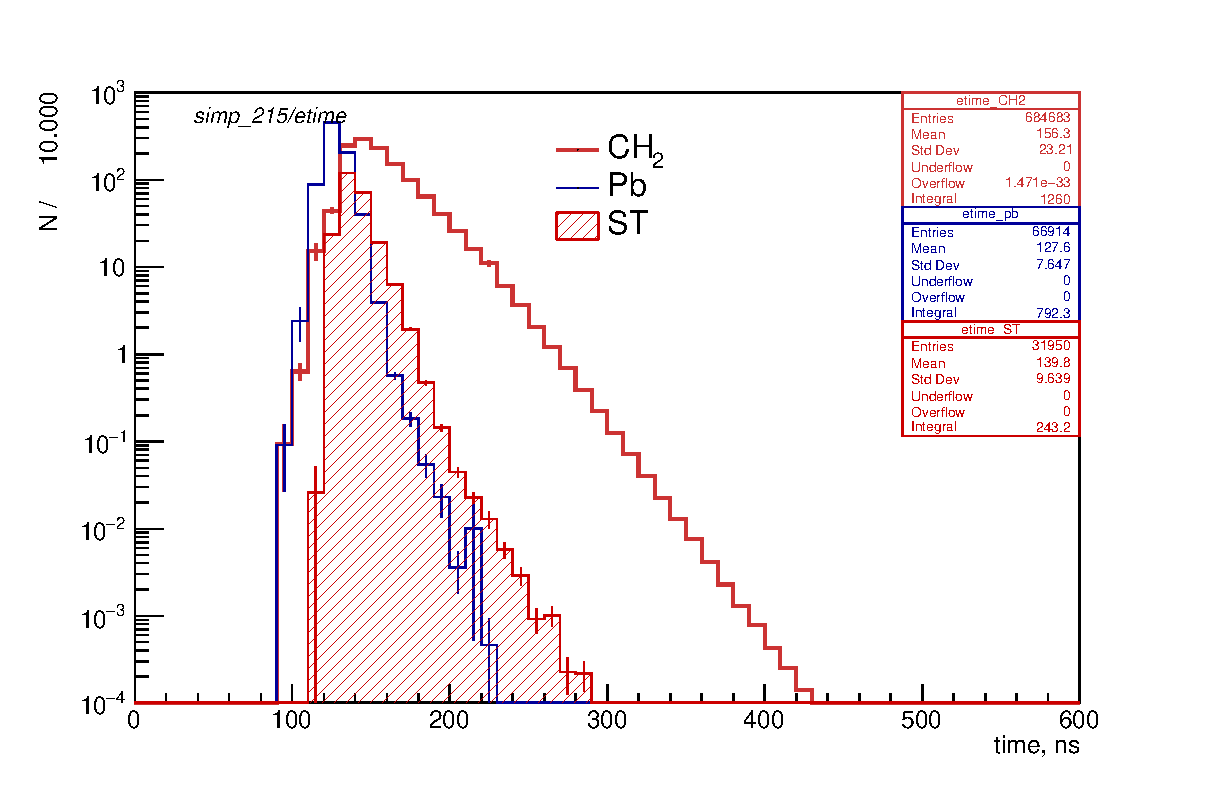
\includegraphics[width=0.5\textwidth]{png/figure_00021}
      % }
    };
    \node[anchor=south west,inner sep=0] at (10,0.) {
      % \node[shift={(0 cm,0.cm)},inner sep=0,rotate={90}] at (0,0) {}
      % \makebox[\textwidth][c] {
        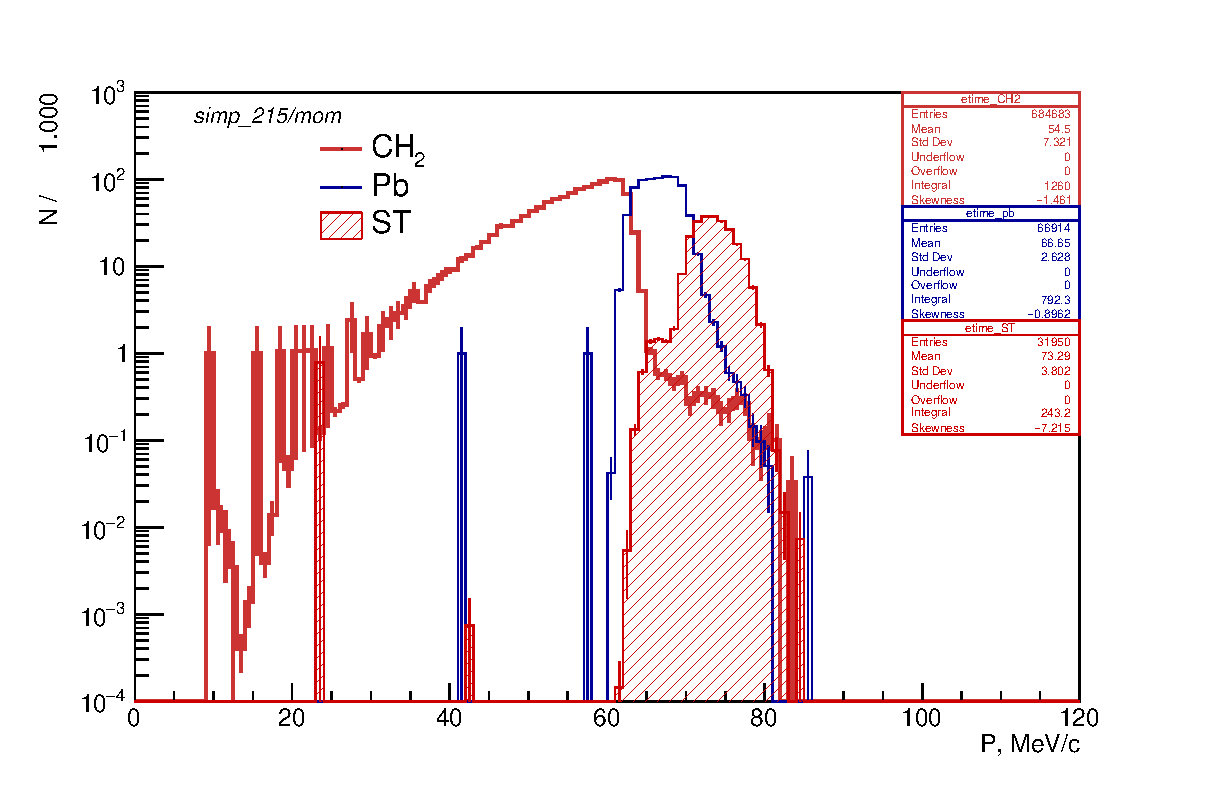
\includegraphics[width=0.5\textwidth]{png/figure_00022}
      % }
    };
    % \node [text width=8cm, scale=1.0] at (14.5,0.5) {$\mu_B$, expected background mean};
    % \node [text width=8cm, scale=1.0, rotate={90}] at (1.5,7.5) { $S_{D}$, ``discovery'' signal strength  };
  \end{tikzpicture}
  \caption{
    \label{figure:sum_mom_vd13}
    Stopped pions: distributions of momentum and time
  }
\end{figure}


Y vs X :

\begin{figure}[H]
  \begin{tikzpicture}
    \node[anchor=south west,inner sep=0] at (0,0.) {
      % \node[shift={(0 cm,0.cm)},inner sep=0,rotate={90}] at (0,0) {}
      %\makebox[\textwidth][c] {
        \includegraphics[width=0.5\textwidth]{png/figure_00034}
      %}
    };
    \node[anchor=south west,inner sep=0] at (10.,0.) {
      % \node[shift={(0 cm,0.cm)},inner sep=0,rotate={90}] at (0,0) {}
      %\makebox[\textwidth][c] {
        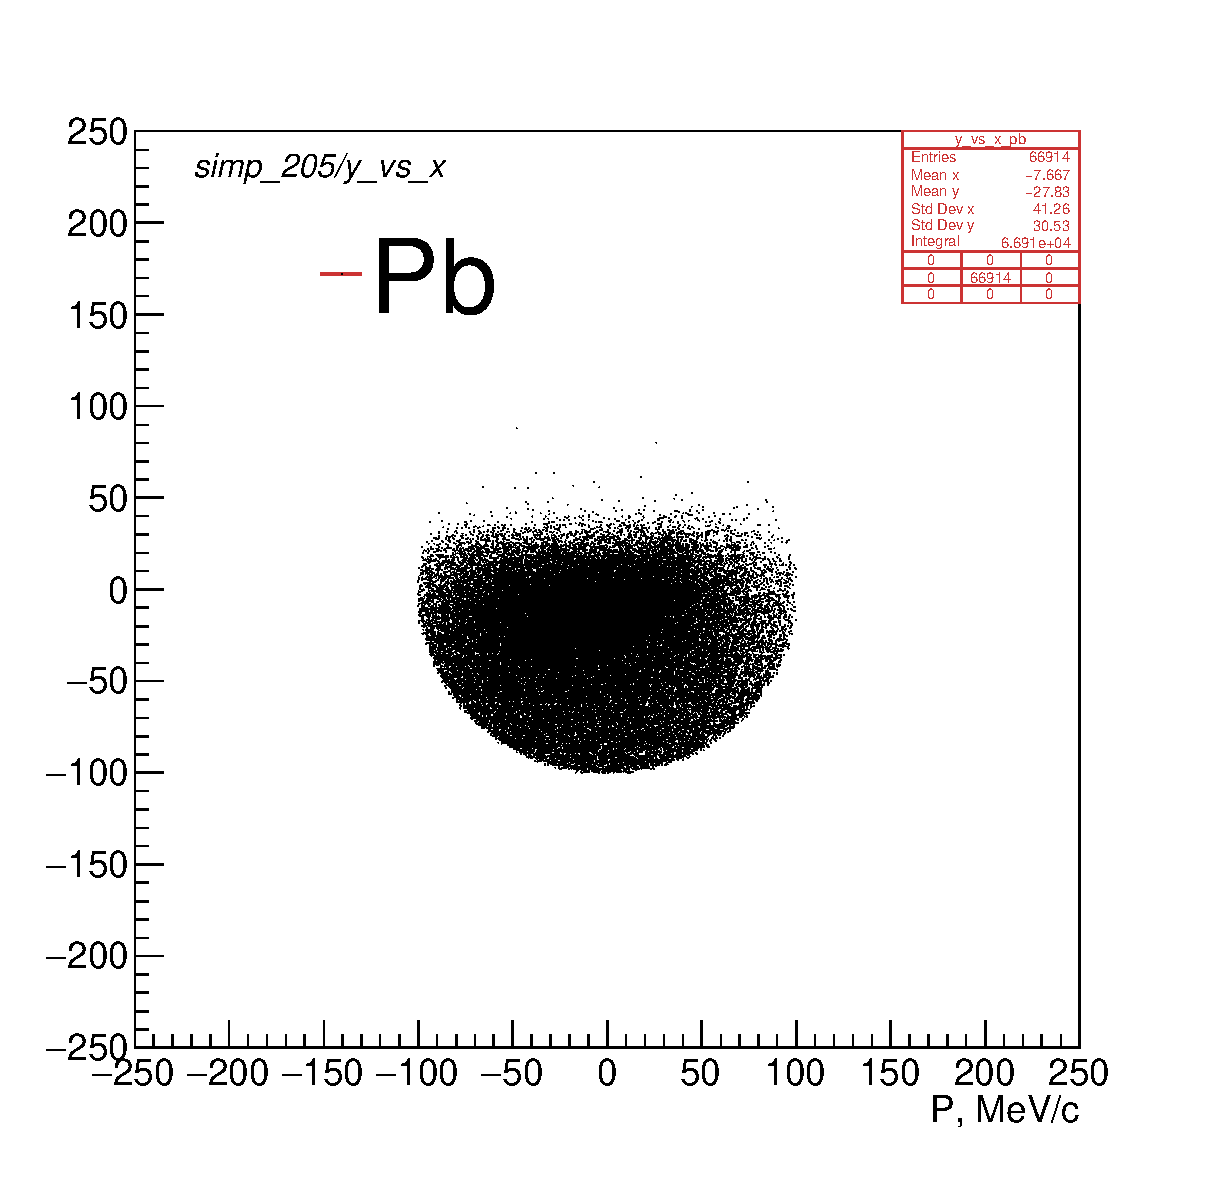
\includegraphics[width=0.5\textwidth]{png/figure_00035}
      %}
    };
    \node[anchor=south west,inner sep=0] at (0,-10.) {
      % \node[shift={(0 cm,0.cm)},inner sep=0,rotate={90}] at (0,0) {}
      % \makebox[\textwidth][c] {
        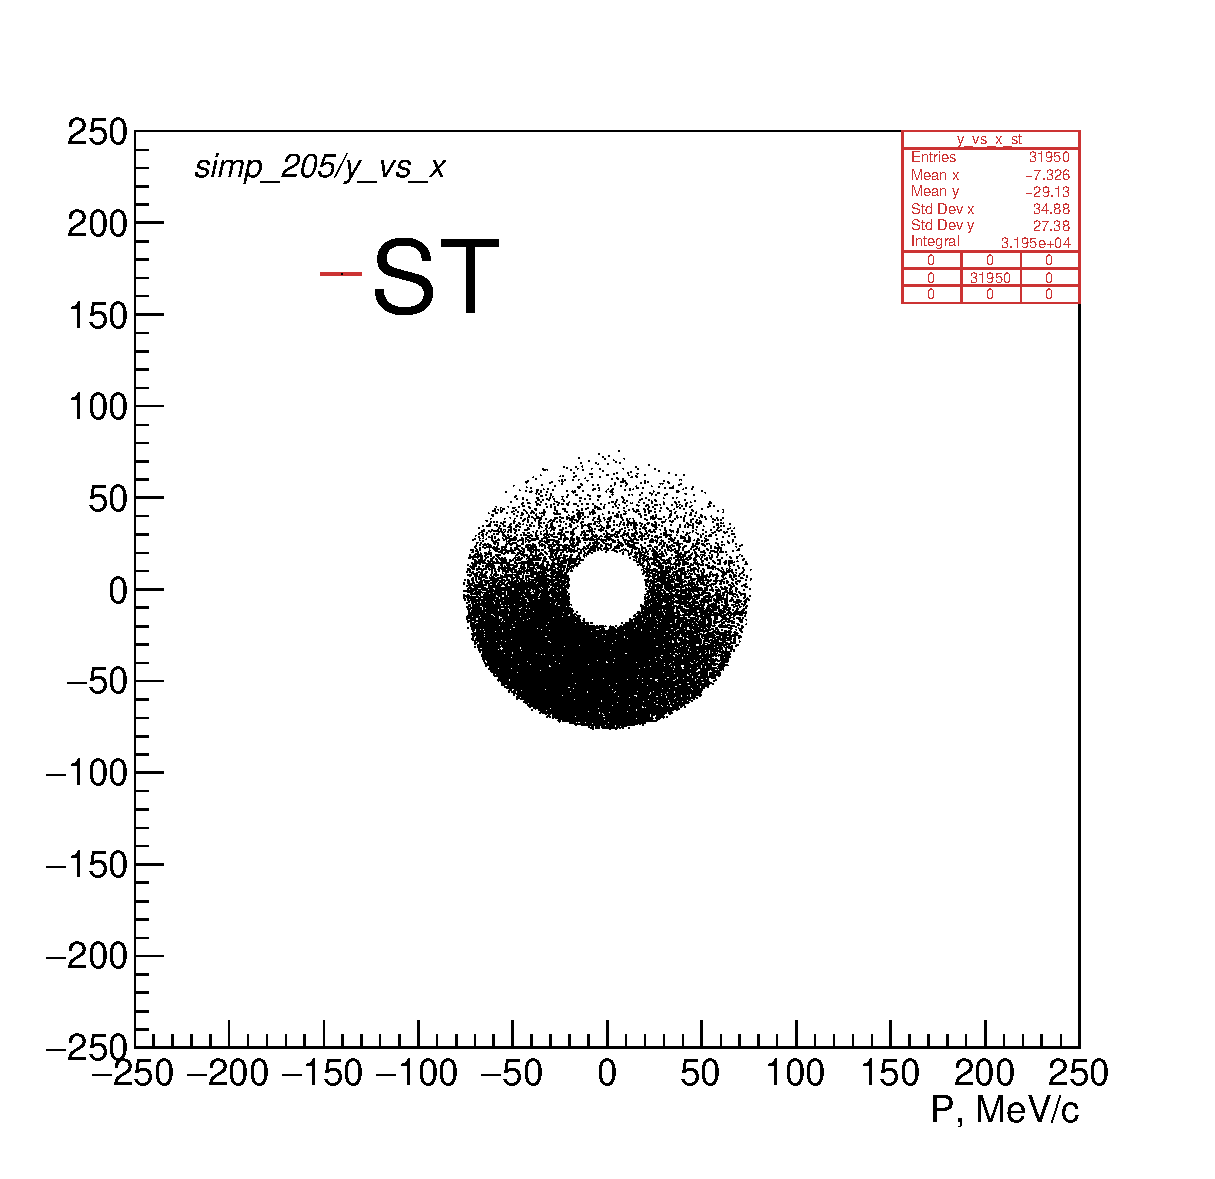
\includegraphics[width=0.5\textwidth]{png/figure_00031}
      % }
    };
    % \node [text width=8cm, scale=1.0] at (14.5,0.5) {$\mu_B$, expected background mean};
    % \node [text width=8cm, scale=1.0, rotate={90}] at (1.5,7.5) { $S_{D}$, ``discovery'' signal strength  };
  \end{tikzpicture}
  \caption{
    \label{figure:y_vs_x_st}
    Y(stop):X(stop) for pions stopped in the CH2 and Pb
  }
\end{figure}

The distributions in Figure \ref{figure:y_vs_x_st} are a consequence of the momentum-dependent vertical
drift of transported particles in the TS, where for particles with momentum above 50 MeV/c the vertical offset
due to the drift in TSd overcompensates the offset due to the drift in TSu.
The correlation between the vertical position of stopped particles in teh degrader and the particle momentum
on exit from the TS is shown in Figure ~\ref{figure:y_vs_p_deg}.

\begin{figure}[H]
  \begin{tikzpicture}
    \node[anchor=south west,inner sep=0] at (0,0.) {
      % \node[shift={(0 cm,0.cm)},inner sep=0,rotate={90}] at (0,0) {}
      %\makebox[\textwidth][c] {
        \includegraphics[width=0.5\textwidth]{png/figure_00036}
      %}
    };
    \node[anchor=south west,inner sep=0] at (10.,0.) {
      % \node[shift={(0 cm,0.cm)},inner sep=0,rotate={90}] at (0,0) {}
      % \makebox[\textwidth][c] {
      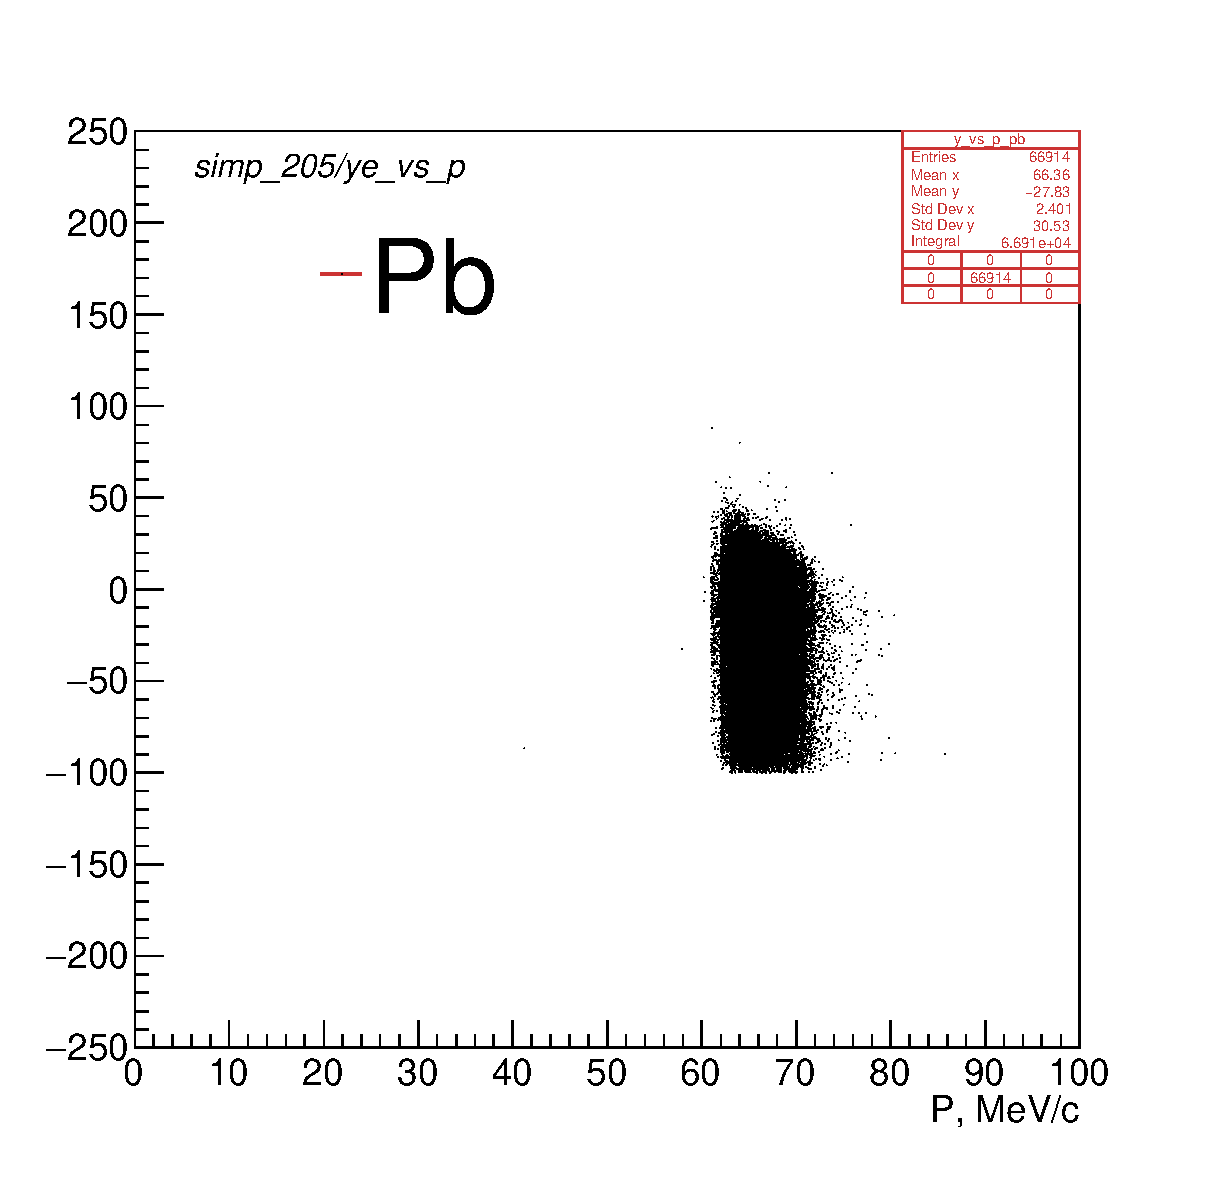
\includegraphics[width=0.5\textwidth]{png/figure_00037}
      % }
    };
    % \node [text width=8cm, scale=1.0] at (14.5,0.5) {$\mu_B$, expected background mean};
    % \node [text width=8cm, scale=1.0, rotate={90}] at (1.5,7.5) { $S_{D}$, ``discovery'' signal strength  };
  \end{tikzpicture}
  \caption{
    \label{figure:y_vs_p_deg}
    Y(stop):P\@(DS entrance) for negative pions stopped in the $CH_2$ and Pb parts of the simulated degrader
  }
\end{figure}


%%% Local Variables:
%%% mode: latex
%%% TeX-master: t
%%% End:
